%!TEX root = ../thesis.tex
\begin{section}{Technical concepts \label{sec:tc}}

In this section we review the technical concepts needed for this thesis. We do not attempt to give detailed summaries of these topics, but rather present some of the key theorems that will be used along with some basic definitions and results required to understand these theorems.

\begin{subsection}{Probability Theory}
	\label{sec:tc:pt}
	Although this thesis, for the most part, does not require a measure-theoretic formalisation of probability theory, we require knowledge of what both a measure space and a $\sigma$-finite measure space is, in order to understand some of the key theorems we shall use.
	This motivates us to discuss some of the basic definitions from measure-theoretic probability.
	\begin{definition}
		If $\Omega$ is a given set, then a \emph{$\sigma$-field} $\mathcal{F}$ on $\Omega$ is a collection of subsets satisfying the following conditions:
		\begin{enumerate}
			\item $\Omega \in \mathcal{F}$,
			\item If $A \in \mathcal{F}$ then $A^c \in \mathcal{F}$,
			\item If a countable sequence $A_1,A_2,\dots \in \mathcal{F}$ then
			\[\bigcup_{i \geq 1} A_i \in \mathcal{F}. \]
		\end{enumerate}
		We call the pair $(\Omega, \mathcal{F})$ a \emph{measurable space}.
	\end{definition}

	\begin{definition}
	Given two measurable spaces $(\Omega_1,\mathcal{F}_1)$ and $(\Omega_2,\mathcal{F}_2)$, a function $X: \Omega_1 \to \Omega_2$ is said to be \emph{measurable} if for every $A \in \mathcal{F}_2$ we have $X^{-1}(A) \in \mathcal{F}_1$.
	\end{definition}

\begin{theorem}
	\label{thm:measurablefunctionproduct}
	If $f$ and $g$ are both measurable functions, then the product of these functions, $fg$, is also measurable.
\end{theorem}
	\begin{definition}
		Let $\Omega$ be a sample space and $\mathcal{F}$ be a $\sigma$-algebra on $\Omega$. A function $\mu: \mathcal{F} \to \mathbb{R} \cup \{-\infty,\infty\}$ is called a \emph{measure} if it satisfies the following properties 
			\begin{enumerate}
			\item $\mu(A) \geq 0$, for all $A$ in $\mathcal{F}$, 
			\item $\mu(\emptyset) = 0$,
			\item For all countable collections $\{A_i\}_{i=1}^\infty$ of pairwise disjoint sets in $\mathcal{F}$,
			\begin{equation*}
			\mu \left(\bigcup_{k=1}^\infty A_k \right)  = \sum_{k=1}^\infty \mu(A_k).
			\end{equation*}
		\end{enumerate}
	\end{definition}
	A natural extension to a measure is the probability measure.
	\begin{definition}
		A measure on a sample space $\Omega$ is called a \emph{probability measure} if the total measure is one, that is $\mu(\Omega) = 1$.
	\end{definition}
	\iffalse
	\begin{definition}[Probability measure]
		A \emph{probability measure} $\P$ on a measurable space $(\Omega, \mathcal{F})$ is a function $\P:\mathcal{F}\to [0,1]$ such that
		\begin{enumerate}
			\item $\P(\Omega) = 1$.
			\item For every infinite sequence $A_1,A_2,\dots \in \mathcal{F}$,
			\[\P\left(\bigcup_i A_i \right) \leq \sum_i \P(A_i). \]
			\item For every mutually exclusive infinite sequence $A_1,A_2,\dots \in \mathcal{F}$,
			\[\P\left(\bigcup_i A_i \right) = \sum_i \P(A_i). \]
		\end{enumerate}
	\end{definition}
	\begin{definition}[Probability space]
		A \emph{probability space} is a triplet $(\Omega,\mathcal{F},\P)$, where $\Omega$ is a sample space $\mathcal{F}$ is a $\sigma$-field on $\Omega$, and $\P:\mathcal{F}\to [0,1]$ is a probability measure on $(\Omega,\mathcal{F})$.
	\end{definition}
\begin{definition}
	An \emph{event} $A \in \mathcal{F}$, has a probability $\P(A)$ of occurring. We say the event happens \emph{almost surely} (a.s.) if $\P(A) = 1$.
\end{definition}
\fi


\iffalse
\begin{definition}
	Given a collection $G$ of subsets of $\Omega$, where $G$ is not necessarily a $\sigma$-field, there is always at least one $\sigma$-field which contains $G$. We define 
	\[\mathcal{F}(G) := \bigcap_{k} \mathcal{F}_k, \]
	where $\{\mathcal{F}_k\}$ are all $\sigma$-fields that contain $G$. We say that the $\sigma$-field $\mathcal{F}(G)$ is \emph{generated} by $G$.
\end{definition}
\begin{definition}[Borel $\sigma$-field]
	The \emph{Borel $\sigma$-field} on $\Omega$, denoted $\mathcal{B}_{\Omega}$, is the $\sigma$-field generated by the set of all closed intervals $[a,b] \in \Omega$.
\end{definition}

Commonly used Borel $\sigma$-fields are $\mathcal{B}_{[0,1]}$, $\mathcal{B}_{\mathbb{R}}$, and $\mathcal{B}_{\mathbb{R}^d}$ which are the Borel $\sigma$-fields on $[0,1]$, $\mathbb{R}$, and $\mathbb{R}^d$, respectively.

\begin{definition}[Random variable]
Let $X$ be a measurable function from the measurable space $(\Omega_1,\mathcal{F}_1)$ to the measurable space $(\mathbb{R},\mathcal{B}_{\mathbb{R}})$, where $\mathcal{B}_{\mathbb{R}}$ is the Borel $\sigma$-field on $\mathbb{R}$, then we say that $X$ is a \emph{random variable}.
\end{definition}
If the second measurable space is instead $(\mathbb{R}^d, \mathcal{B}_{\mathbb{R}^d})$, then we say that $X$ is a \emph{$d$-dimensional random vector}.

\begin{definition}[Probability distribution]
	Given a probability space $(\Omega, \mathcal{F},\P)$ and a random variable $X : \Omega \to \mathbb{R}$, the associated \emph{probability distribution} is defined to be the function $F: \mathbb{R} \to [0,1]$ given by
	\[F(x): \P(\omega \in \Omega : X(\omega) \leq x). \]
	If $F(x)$ is differentiable, then its derivative
	\[f(x): = \frac{d}{dx} F(x) \]
	is called a \emph{density function}.
\end{definition}
\fi
\begin{definition}
	Let $\mu$ be a measure on the measurable space $(\Omega,\mathcal{F})$. Then we say that $(\Omega,\mathcal{F},\mu)$ is a \emph{measure space}.
\end{definition}
\begin{definition}
	A measure $\mu$ on a measurable space $(\Omega,\mathcal{F})$ is called a \emph{finite measure} if it satisfies
	\begin{equation*}
	\mu(A) < \infty,
	\end{equation*}
	for all $A \in \mathcal{F}$.
\end{definition}

\begin{definition}
	\label{def:sigmafinitemeasure}
	Let $\mu$ be a measure on the measurable space $(\Omega,\mathcal{F})$. We say that $\mu$ is a \emph{$\sigma$-finite measure} if the set $\Omega$ is the countable union of sets with finite measure.
\end{definition}
For example, the Lebesgue measure on the real numbers is a $\sigma$-finite measure but not a finite measure. To see this, consider an interval $[k,k+1)$ which has a measure of $1$, since the Lebesgue measure for an interval is defined as its width, $\mu([a,b]) = b-a$. The real numbers can be constructed by a countable union of intervals of this form, and so by \cref{def:sigmafinitemeasure} is $\sigma$-finite. However, the Lebesgue measure of the real numbers, $\mu\left( (-\infty,\infty) \right)$ is not finite.

Another example we can consider is the counting measure, which for any finite set is the number of elements in that set. Clearly, this measure is neither finite nor $\sigma$-finite for $\mathbb{R}$. However, the set $\mathbb{N}$ is countable and the counting measure is $\sigma$-finite.
\begin{definition}
	If $\mu$ is a $\sigma$-finite measure, then we say that $(\Omega,\mathcal{F},\mu)$ is a \emph{$\sigma$-finite measure space}.
\end{definition}
Finally, we present a theorem that will be used frequently throughout the thesis, which uses the definitions presented above.
\begin{theorem}[Tonelli's Theorem]
	\label{thm:tonellistheorem}
	If $(X,\mathcal{A},\mu)$ and $(Y,\mathcal{B},\nu)$ are $\sigma$-finite measure spaces and $f:X \times Y \to [0,\infty)$ is non-negative and measurable, where $X \times Y$ is given the product measure (which is unique since $X$ and $Y$ are $\sigma$-finite), then
	\begin{equation*}
	\label{eq:tonelli}
	\int_X \left( \int_Y f(x,y)\nu(dy) \right) \mu(dx) = \int_Y \left( \int_X f(x,y)\mu(dx) \right) \nu(dy) = \int_{X \times Y} f d \mu \times \nu.
	\end{equation*}
\end{theorem}
	\Myref{thm:tonellistheorem} allows us to rearrange the order of integration or summation under certain circumstances. 
	Using some of the above definitions, we can show some specific circumstances in which Tonelli's theorem will hold, in order to avoid discussion of measure-theory throughout the thesis.
	
	\begin{corollary}
		\label{thm:switchintegrals}
		If $g(x,y)$ and $h(x,y)$ are two non-negative and measurable functions on $X \times Y$ where $X=[a,b]$ and $Y=[c,d]$ for some $a,b,c,d \in \mathbb{R}$, then
		\begin{equation*}
		\int_{a}^b \int_c^d g(x,y)h(x,y)dydx = \int_{c}^d \int_{a}^b g(x,y)h(x,y)dxdy.
		\end{equation*}
	\end{corollary}
\begin{proof}

	Both $g(x,y)$ and $h(x,y)$ are non-negative and measurable and so if we define $f(x,y) = g(x,y)h(x,y)$, then $f(x,y)$ will be a non-negative and measurable function, according to \cref{thm:measurablefunctionproduct}. Both $(X,\mathcal{B}_{X})$ and $(Y,\mathcal{B}_{Y})$ are measurable spaces, where $\mathcal{B}_{X}$ and $\mathcal{B}_{Y}$ are the Borel $\sigma$-algebras generated by $[a,b]$ and $[c,d]$ respectively. Then, we can construct $(X,\mathcal{B}_{X}, \mu)$ and $(Y,\mathcal{B}_{Y},\mu)$ where $\mu$ is the Lebesgue measure, which are both $\sigma$-finite measure spaces. Therefore, we can apply \myref{thm:tonellistheorem} to arrive at the desired result.
\end{proof}
	Note that a \ac{PDF} by definition will be a non-negative and measurable function, so if $g(x,y)$ and $h(x,y)$ are both \acp{PDF} they must both satisfy the conditions of \cref{thm:switchintegrals}.
\begin{corollary}
	\label{thm:switchsummations}
	If $g(x,y)$ and $h(x,y)$ are two non-negative and measurable functions on $X \times Y$ where $X$ and $Y$ are both subsets of the natural numbers, then
	\begin{equation*}
	\sum_{X} \sum_Y g(x,y)h(x,y) = \sum_{Y} \sum_{X} g(x,y)h(x,y).
	\end{equation*}
\end{corollary}
	\begin{proof}
	The proof is exactly the same as that of \cref{thm:switchintegrals}, but we instead define $\mu$ as the counting measure.
\end{proof}
For example, using \cref{thm:switchsummations} we could get the following
\begin{equation*}
\sum_{x=0}^\infty \sum_{y=0}^n g(x,y)h(x,y) = \sum_{y=0}^n \sum_{x=0}^\infty g(x,y)h(x,y).
\end{equation*}
\begin{corollary}
	\label{thm:switchsummationintegral}
If $g(x,y)$ and $h(x,y)$ are two non-negative and measurable functions on $X \times Y$ where $X = [a,b]$ for $a,b \in \mathbb{R}$ and $Y$ is s subset of the natural numbers, then
\begin{equation*}
\sum_{Y} \int_a^b g(x,y)h(x,y)dx = \int_{a}^b \sum_{Y} g(x,y)h(x,y)dx.
\end{equation*}
\end{corollary}
This \lcnamecref{thm:switchsummationintegral} is simply a combination of \cref{thm:switchintegrals,thm:switchsummations}, allowing us to switch the the ordering of integrals and summations.

Note that \Myref{thm:tonellistheorem} can be applied multiple times in order to rearrange an expression on more than two measure spaces, as long as the same conditions are met such as the functions all being non-negative and measurable. This also means that \cref{thm:switchintegrals,thm:switchsummations,thm:switchsummationintegral} can be applied to switch the order of integration and summation of an arbitrary number of non-negative and measurable functions.

\end{subsection}
\subsection{Stochastic processes}

Now, we discuss some basic stochastic processes that will be used throughout this thesis, as well as some of their properties.
Most important is the random walk.

\begin{definition}
	\label{def:tc:stochastic:randomwalk}
	Let $\{X_k\}_{k=1}^\infty$ be a sequence of independent, identically distributed random variables. For every positive $n$, we denote
	\begin{equation*}
	 S_n = \sum_{k=1}^n X_k.
	 \end{equation*}
	The sequence $\{S_n\}_{n=1}^\infty$ is called a \emph{random walk}.
\end{definition}

In other words, a random walk is a stochastic process describing a path of successive random steps on some mathematical space.
In \cref{sec:1dRW} we use random walks to represent the movement of an animal, with the distribution of $X_k$ affecting the strategy that is used.
Although the random walk is a discrete-time process, it has a strong relationship to some continuous-time processes, such as the Wiener process, which is also referred to as Brownian motion.
\begin{definition}
	A Brownian motion $\mathcal{B} = \{B_t\}_{t\geq 0}$ with variance $\sigma^2$ is a stochastic process that satisfies the following properties:
	\begin{enumerate}
		\item $B_0 = 0$ almost surely.
		\item $\mathcal{B}$ has independent increments: for $0 \leq t_1 < \dots < t_k < \infty$ and $x_1,x_2,\dots,x_k \in \mathbb{R}$,
		\begin{align*}
		\Pr &\left( B_{t_2}-B_{t_1} \leq x_1, B_{t_3}-B_{t_2} \leq x_2, \dots, B_{t_k} - B_{t_{k-1}} \leq x_{k-1} \right)\\
		 &= \prod_{2 \leq i \leq k} \Pr \left(B_{t_i} - B_{t_{i-1}} \leq x_{i-1} \right).
		 \end{align*}
		 \item For every $0 \leq s \leq t$, $B_t - B_s \sim N(0,\sigma^2(t-s))$ --- stationary, Gaussian increments with variance $\sigma^2(t-s)$.
		 \item $\mathcal{B}$ has continuous sample paths, almost surely.
	\end{enumerate}
We use $\mathcal{B}\left(\mu,\sigma^2\right)$ to denote a Brownian motion with drift $\mu$ and variance $\sigma^2$, where the drift represents the expected increase or decrease per unit time. A Brownian motion with a drift of $0$ and a variance of $1$, denoted $\mathcal{B}(0,1)$, is known as a \emph{standard Brownian motion}.
\end{definition}

Recall the \ac{CLT}, which gives conditions under which a sequence of properly normalised random variables will converge to a normal distribution.
\begin{theorem}[Central Limit Theorem]
	If $\E{X_1} = \mu$, $\Var{X_1} = \sigma^2 \in (0,\infty)$, and $S_n = X_1 + \dots +X_n$, with $X_i$ i.i.d., then
	\begin{equation*}
	\frac{S_n - n \mu}{\sqrt{n}\sigma} \to N(0,1) \text{ as }n \to \infty
	\end{equation*}
	in distribution.
\end{theorem}
Note that the \ac{CLT} requires a finite variance, and so will not apply to heavy-tailed distributions. We now introduce a functional extension of the \ac{CLT}, which can be used to investigate the continuous-time limit of a random walk.

\begin{theorem}[Donsker's Theorem]	
	\label{thm:donskers_theorem}
Consider a random walk, $S_n$, with i.i.d. steps $X_i$ such that $\E{X_i} = 0$ and $\Var{X_i}=1$. We define
\begin{equation}
W^{(n)}(t): = \frac{S_{\floor{nt}}}{\sqrt{n}}.
\end{equation}
Then, Donsker's invariance principle \cite{Donsker_1952} states that 
$W^{(n)}(1) \to \mathcal{B}$ in distribution as $n \to \infty$, where $\mathcal{B}$ denotes a standard Brownian motion.
\end{theorem}

%The Skorokhod space $\mathcal{D}[0,1]$ is simply the collection of càdlàg (right continuous with left limits) functions on the domain $[0,1]$. 

Now, although an expectation of $0$ and variance of $1$ is required for this to apply, in general we can rescale our random variable as long as these are not infinite.
Thus, just like the \ac{CLT}, Donsker's Theorem is not valid for heavy-tailed distributions.
In the following example, we consider an unbounded power-law distribution and show at what values Donsker's Theorem will apply, and how we can rescale to make the variance $1$.

\begin{example}
	\label{ex:donskers}
	Let $X$ be a random variable with unbounded power-law distribution centred about $0$, which has density function
	\begin{equation*}
	p(x) = \frac{\mu-1}{2 x_{\min}}\left(\frac{\lvert x \rvert }{x_{\min}}\right)^{-\mu}, \quad \lvert x \rvert \in [x_{\min},\infty), \quad x_{\min} > 0, \quad \mu > 1.
	\end{equation*}
	The $m$th moment of $X$ is given by
	\begin{align*}
	\E{X^m} &= \int_{-\infty}^{-x_{\min}}x^m p(x) dx + \int_{x_{\min}}^\infty x^m p(x) dx\\
	&= \frac{\mu-1}{2} x_{\min}^{\mu-1} \left( \int_{-\infty}^{-x_{\min}} x^m(-x)^{-\mu} dx + \int_{x_{\min}}^\infty x^{-\mu +m} dx \right).
	\end{align*}
	Then, if $m < \mu - 1$, we get
	\begin{align*}
	\E{X^m} &= \frac{\mu-1}{2} x_{\min}^{\mu-1} \left ( \left[\frac{x^{m+1}(-x)^{-\mu}}{-\mu+m+1}\right]^{-x_{\min}}_{-\infty} +\left[\frac{x^{-\mu+m+1}}{-\mu+m+1}\right]_{x_{\min}}^{\infty} \right)\\
		&= \frac{\mu-1}{2(\mu-1-m)} \left( x_{\min}^{m} + (-x_{\min})^{m} \right).
	\end{align*}
	For $m \geq \mu - 1$, the $m$th moment is undefined. Based on the above, the first moment is $\E{X}=0$ for all $\mu \geq 2$. The second moment, and hence the variance, will be
	\begin{equation*}
	\Var{X} = \E{X^2} = \begin{cases}
	\displaystyle \frac{\mu-1}{\mu-3} x_{\min}^2 \quad &\text{for } \mu > 3,\\
	\text{undefined} \quad &\text{for }\mu \leq 3.
	\end{cases}
	\end{equation*}
	
	Since $\E{X}=0$, we do not need to shift $X$, although we do need to scale $X$ to account for $\Var{X} \neq 1$. For $\mu > 3$, we define
	\begin{equation*}
	Y:= \sqrt{\frac{\mu-3}{\mu-1} x_{\min}^{-2}} X,
	\end{equation*}
	so $\E{Y}=0$ and $\Var{Y}=1$. Therefore, using Donsker's Theorem, a random walk $S^{(y)}_n$ with i.i.d steps, $Y_i$, will converge in distribution to a standard Brownian motion.
	
	Thus, we can also say that the random walk $S^{(x)}_n$ with i.i.d steps, $X_i$, will converge in distribution to the Brownian motion  $\mathcal{B}\left(0,  \frac{\mu-1}{\mu-3} x_{\min}^2  \right)$ for $\mu > 3$. Similarly, when $\mu=3$, $S_n^{(x)}$ will converge in distribution to the Brownian motion $\mathcal{B}\left(0,  2 \log(x_{\min}) x_{\min}^2  \right)$.
\end{example}

As we have just shown in \cref{ex:donskers}, the unbounded power-law distribution converges to a Brownian motion for $\mu \geq 3$, but does not for $1 < \mu < 3$ since the distribution will be heavy-tailed.


\subsection{Point processes}
In \cref{sec:2dmodel}, we investigate a two-dimensional model where food targets are randomly distributed over a two-dimensional space.
Point processes are collections of points on some mathematical space, and are often used to model physical objects that can be represented as a point in space.
Thus, point processes are an obvious choice to represent our food targets.
Further, we use the simplest and most ubiquitous point process, which is the Poisson point processes.

\begin{definition}
	A \emph{Poisson point process} is a collection of points randomly located on some underlying mathematical space, where the number of points in one subregion is independent of the number of points in any other disjoint subregion. We call this property \emph{complete randomness}.
\end{definition}
	
	For a Poisson point process, the number of points, $N$, in a bounded region is given by a Poisson distribution:
	\[\Pr(N=n) = \frac{\Lambda^n}{n!}e^{-\Lambda}, \]
	where the parameter $\Lambda$ is determined by the region. The parameter $\Lambda$ is also the expected value of $N$.

A further simplification we can make is to consider homogeneous Poisson point processes.

\begin{definition}
	If a Poisson point process has a parameter of the form $\Lambda = \nu \lambda$, where $\nu$ is Lebesgue measure, and $\lambda$ is a constant, then we say that the Poisson point process is \emph{homogeneous} or \emph{stationary}.
\end{definition}
Since Lebesgue measure assigns length, area, or volume to a set, then $\lambda$ can be considered the mean number of points per some unit, usually length, area, or volume, depending on the underlying mathematical space.

For our purposes, we only consider Poisson point processes that are two-dimensional.

\begin{definition}
	\label{def:spatialpoisson}
	A \emph{spatial Poisson point process}, $\mathcal{N}$, is a Poisson point process defined in the plane $\mathbb{R}^2$.
\end{definition}


\subsection{Linear operators and norms}
Throughout \cref{sec:1Dmodel}, we use linear operators to deal with each step that a forager takes. We also need to prove some properties about operators, such as their norm. This motivates us to give a brief summary of linear operators and norms.
\begin{definition}
	Given a vector space $V$, a \emph{norm} on $V$ is a non-negative scalar function $f:V\to [0,\infty)$ with the properties:
	For all $a \in \mathbb{R}$ and all $\vec{u}$, $\vec{v} \in V$,
	\begin{enumerate}
		\item $f(\vec{u}+\vec{v}) \leq f(\vec{u}) + f(\vec{v})$,
		\item $f(a\vec{v}) = \left| a\right| f(\vec{v})$,
		\item If $f(\vec{v}) = 0$ then $\vec{v}=\vec{0}$.
	\end{enumerate}
\end{definition}
A norm assigns some positive length or size to vectors that are in a vector space, except for the zero vector which is assigned zero.
Some of the most widely used norms are the $1$-norm, $2$-norm, and $\infty$-norm, which are all cases of the $p$-norm.
\begin{definition}
	The $p$-norm, denoted $\norm{\cdot}_p$ of a vector $\vec{v} \in V$ is defined as
	\begin{equation*}
	\norm{\vec{x}}_p = \left( \lvert x_1 \rvert^p + \cdots + \lvert x_n \rvert^p \right)^{1/p}
	\end{equation*}
	for $p \geq 1$, $\vec{x} \in \mathbb{R}^n$, $V = \mathbb{R}^p$.
\end{definition}

Then, the $1$-norm is
\begin{equation*}
\norm{\vec{x}}_1 = \lvert x_1 \rvert + \cdots + \lvert x_n \rvert,
\end{equation*}
the $2$-norm is
\begin{equation*}
\norm{\vec{x}}_2 = \sqrt{\lvert x_1 \rvert^2 + \cdots + \lvert x_n \rvert^2},
\end{equation*}
and the $\infty$-norm is
\begin{equation*}
\norm{\vec{x}}_\infty = \lim_{p \to \infty} \norm{\vec{x}}_p  =\max_{1 \leq i \leq n} \lvert x_i \rvert.
\end{equation*}

We can also talk about the norm of a matrix rather than a vector.

\begin{definition}
	Given a real matrix $A$, a matrix norm $\norm{A}$ is a non-negative number associated with $A$ having the properties
	\begin{enumerate}
		\item $\norm{A} \geq 0$ with equality iff $A = 0$,
		\item $\norm{kA} = \lvert k \rvert \norm{A}$ for any scalar $k$,
		\item $\norm{A+B} \leq \norm{A} + \norm{B}$,
	\end{enumerate}
\end{definition}

As with the vector norm, their exists a matrix $p$-norm.
\begin{definition}
	The $p$-norm of a matrix, denoted $\norm{\cdot}_p$, is defined as
	\begin{equation*}
	\norm{\vec{x}}_p = \max_{\norm{x}_p=1} \norm{ A \vec{x} }_p,
	\end{equation*}
	for $p \geq 1$, and where $\norm{\vec{x}}_p$ is the vector $p$-norm.
\end{definition}
The $1$-norm is the maximum absolute column sum, 
\begin{equation*}
\norm{A}_1 = \max_{1 \leq j \leq m} \sum_{i=1}^n \lvert a_{ij} \rvert,
\end{equation*}
where $A$ has dimensions $n \times m$, and the $\infty$-norm is the maximum absolute row sum,
\begin{equation*}
\norm{A}_\infty = \max_{1 \leq i \leq n}\sum_{j=1}^m \lvert a_{ij} \rvert.
\end{equation*}

A natural generalisation of the $p$-norm for finite-dimensional vector spaces is the $L^p$-norm for function spaces.

\begin{definition}
	On a measure space $(X,\mathcal{F},\mu)$, the $L^p$-norm of a function $f: X \to \mathbb{R}$ is 
	\begin{equation*}
	\norm{f}_{L^p} = \left(\int_X \lvert f \rvert^p d \mu \right)^{1/p} .
	\end{equation*}
\end{definition}


\begin{definition}
	\label{def:linear_map}
	Let $V$ and $W$ be vector spaces. A function $f: V \to W$ is said to be a \emph{linear map} (or linear transformation) if for any two vectors $\vec{u}, \vec{v} \in V$ and any scalar $c \in \mathbb{R}$ the following conditions are satisfied:
	\begin{enumerate}
		\item $f(\vec{u}+\vec{v}) = f(\vec{u}) + f(\vec{v})$,
		\item $f(c\vec{u}) = cf(\vec{u})$.
	\end{enumerate}
\end{definition}
For example, an integral over some interval $I$ is a linear map from the space of all real-valued integrable functions on $I$ to $\mathbb{R}$. The expectation of a random variable is also a linear map, but the variance of a random variable is not since it is not linear.
\begin{definition}
	\label{def:linear_operator}
	A \emph{linear operator} is a linear map as defined in \cref{def:linear_map}, with $V=W$.
\end{definition}

\begin{definition}
	\label{def:bounded_linear_operator}
	A \emph{bounded} linear operator is a linear operator $T: X \to Y$ for which there exists an $M\geq 0$ such that
	\begin{equation}
	\frac{\norm{Tv}_Y}{\norm{v}_X} \leq M < \infty.
	\end{equation}
\end{definition}

\begin{definition}
	\label{def:neumannseries}
	A Neumann series is a series of the form
	\[\sum_{k=0}^\infty T^k,\]
	where $T$ is an operator and $T^k$ represents $k$ consecutive operations of $T$. Under certain conditions, the convergence of a Neumann series is guaranteed. We discuss this further in \cref{thm:neumann_convergence}
\end{definition}
We can also consider the norm of an operator.
\begin{definition}
	\label{def:operator_norm}
	The operator norm of a linear operator $T:V\to W$ is given by
	\begin{equation*}
	\normop{T} = \sup \left\{\frac{\norm{Tv}}{\norm{v}} : v \in V \text{ with } v \neq 0\right\},
	\end{equation*}
	where the numerator's norm is on $W$ and the denominator's norm is on $V$.
\end{definition}
There are other equivalent definitions of the operator norm, such as
\begin{equation*}
\normop{T} = \inf \left\{ c \geq 0 :  \norm{Tv} \leq c \norm{v} \text{ for all }v \in V   \right\},
\end{equation*}
although we will use the \cref{def:operator_norm} throughout this thesis. Note that each pair of norms on $V$ and $W$ will induce an operator norm.

Intuitively, the operator norm tells us the ``size'' of $T$ by how much it ``stretches'' a vector in the ``biggest'' case.
When $V$ and $W$ are function spaces case we generally use $L^p$-norms in \Cref{def:operator_norm}.
If the operator norm is less than $1$, it will always shrink the vector it is acting on.
Thus, it makes sense that the operator norm will tell us about the convergence of a Neumann series.

\begin{theorem}
	\label{thm:neumann_convergence}
	If $V$ is a Banach space, and the linear operator $T: V \to W$ has $\normop{T} <1$, then convergence of the Neumann series $\sum_{k=1}^\infty T^k $ is guaranteed \cite{Suzuki_1976}.
\end{theorem}

To make sense of this \lcnamecref{thm:neumann_convergence}, we first need to know what a Banach space is.
\begin{definition}
	A Banach space is a complete normed vector space.
\end{definition}
That is, a Banach space is a vector space with a norm defined on it, and is complete in the sense that a Cauchy sequence of vectors always converges to a well-defined limit in the space.
For example, $\mathbb{R}^n$ together with the $p$-norm is a Banach space. Similarly, the Riesz–Fischer theorem \cite{Dunford_1958} tells us that $L^p$ spaces are complete. For the entirety of our thesis we will be considering spaces that are known to be Banach spaces, and so only need to show that the operator norm is less than $1$ to establish convergence.

Establishing the convergence of a Neumann series is important throughout this thesis, since it will allow us to write our expressions without an infinite summation, as the following theorem demonstrates.
\begin{theorem}
	\label{thm:neumannseries}
	Suppose that $T$ is a bounded linear operator on the normed vector space space $V$. If the Neumann series for $T$ converges in the operator norm, then $\Id - T$ is invertible and its inverse is the series
	\[(\Id - T)^{-1} = \sum_{k=0}^\infty T^k, \]
	where $\Id$ is the identity operator in $V$.
\end{theorem}
For a simple, and non-rigorous explanation of why this \lcnamecref{thm:neumannseries} is true, we can consider the partial sums given by
\[S_n := \sum_{k=0}^n T^k.\]
If $T$ converges in the operator norm, then
\begin{align*}
\lim_{n \to \infty} (\Id - T)S_n &= \lim_{n \to \infty} \left( \sum_{k=0}^n T^k - \sum_{k=0}^n T^{k+1} \right)\\
&=\lim_{n \to \infty} \left( \Id - T^{n+1}\right)\\
&=\Id,
\end{align*}
where we used the fact that $\lim_{n \to \infty} T^{n+1} = 0$ if $\normop{T}<1$.
Rearranging gives us
\begin{equation*}
\lim_{n \to \infty} S_n = (\Id - T)^{-1}.
\end{equation*}

We now present a \lcnamecref{thm:composeoperators} about the operator norm of a composition of operators.
\begin{theorem}
	\label{thm:composeoperators}
	If $V$, $W$, and $X$ are three normed spaces and $A: V \to W$ and $B: W\to X$ are bounded operators, then
	\begin{equation*}
	\normop{BA} \leq \normop{B}\normop{A}.
	\end{equation*} 
\end{theorem}

A concept that we also use is the adjoint of an operator.
\begin{definition}
	For a linear operator $A:V\to W$, the \emph{adjoint} operator, denoted $A^*:W\to V$, is an operator that satisfies
	\begin{equation*}
	\langle Av, w \rangle = \langle v, A^* w \rangle,
	\end{equation*}
	for all $v \in V$ and $w \in W$, where $V$ and $W$ are vector spaces with inner products, and $\langle \cdot,\cdot \rangle$ denotes the inner product.
\end{definition}

The following theorem follows from the uniqueness of the adjoint operator.
\begin{theorem}
	For a linear operator $A:V \to W$ with adjoint $A^*:W \to V$ and $B:W\to X$ with adjoint $B^*:X \to W$, 
	\begin{equation*}
	\left(AB\right)^* = B^* A^*.
	\end{equation*}
\end{theorem}

\begin{definition}
	A linear operator $A$ is \emph{self-adjoint} if $A=A^*$.
\end{definition}

Throughout this thesis, the operators that we consider are either matrices or integral operators, and so we discuss some relevant properties of these now.

\begin{theorem}
	The adjoint of a real-valued matrix $A$ is given by its matrix transpose, $A^\top$.
\end{theorem}
\begin{corollary}
	A symmetric matrix is self-adjoint.
\end{corollary}

The integral operators that we use throughout this thesis take the form of a specific integral equation, known as a Fredholm integral.

\begin{definition}
	A Fredholm operator, $A$, takes the form
	\begin{equation}
	\label{eq:fredholm}
	[Af](t)  = \int_a^b K(t,s)f(s)ds,
	\end{equation}
	where $K(t,s)$ is continuous and is referred to as the kernel.
\end{definition}
\begin{theorem}
	The adjoint of the Fredholm operator, $A$, defined in \cref{eq:fredholm} is given by
	\begin{equation*}
	[A^* f](t)  = \int_a^b \overline{K(s,t)}f(s)ds			,
	\end{equation*}
	where $\overline{K(s,t)}$ is the complex conjugate.
\end{theorem}
\begin{corollary}
	\label{thm:fredholmselfadjoint}
	A Fredholm operator with a Hermitian kernel, that is $\overline{K(s,t)} = K(t,s)$, is a self-adjoint operator.
\end{corollary}

We present two more properties about the operator norm of adjoint operators, which we will use multiple times throughout \cref{sec:1Dmodel,sec:1d_discrete}.

\begin{theorem}
	\label{thm:adjointnorm}
	If $A:V\to V$ is a linear operator and $A^* : V \to V$ is its adjoint, then:
	\begin{itemize}
		\item $\normop{A} = \normop{A^*}$,
		\item $\normop{A A^*} = \normop{A}\normop{A^*}$.
	\end{itemize} 
\end{theorem}

Finally, we use these properties to prove a \lcnamecref{thm:selfadjointcomposed} that we will use in this thesis.

\begin{theorem}
	\label{thm:selfadjointcomposed}
	For some self-adjoint linear operator $A:V\to V$, the operator composed with itself $2^n$ times is also self-adjoint where $n$ is a positive integer. That is,
	\begin{equation*}
	A^{2^n} = (A^{2^n})^*.
	\end{equation*}
\end{theorem}
\begin{proof}
	We prove this by induction. For $n=1$, we get
	\begin{equation*}
	A^2 = A A = A^* A^* = (A^*)^2.
	\end{equation*}
	We assume that $A^{2^n} = (A^{2^n})^*$ for some $n>1$ and now consider $A^{2^{n+1}}$.
	\begin{align*}
	A^{2^{n+1}} &= A^{2^n} A^{2^n}\\
	&= \left(A^{2^n}\right)^* \left(A^{2^n}\right)^*\\
	&= \left(A^{2^{n+1}}\right)^*,
	\end{align*}
	where the second line follows from the induction hypothesis. 
\end{proof}
The following \lcnamecref{thm:composedopnorm} follows from \cref{thm:selfadjointcomposed,thm:adjointnorm}.
\begin{corollary}
	\label{thm:composedopnorm}
	For some self-adjoint linear operator $A:V \to V$, $\normop{A^{2^n}} = \normop{A}^{2^n}$, where $n$ is a positive integer.
\end{corollary}
\iffalse
\begin{definition}
	\label{def:levyprocess}
	A right-continuous process $X_t$, $t \in \R_+$, with stationary independent increments is called a Levy process.
\end{definition}

\begin{theorem}
	\label{thm:lindeberg-levy}
	If $\sigma^2 = \Var{Y_1} < \infty$, then
	\[ \frac{S_n - \E{S_n}}{\sqrt{n}} \to Z \sim N(0,\sigma^2)\]
	in distribution as $n \to \infty$.
\end{theorem}

\begin{theorem}
	\label{thm:donker}
	If $\sigma^2 = \Var{Y_1} < \infty$, then for $t\geq 0$
	\[X_t^{(n)} = \frac{S_{[nt]} - \E{S_{[nt]}}}{\sqrt{n}} \to X_t \sim N(0,\sigma^2 t)\]
		in distribution.
		Furthermore, $X^{(n)} \to X$ where $X$ is Brownian motion with diffusion coefficienct $\sigma$.
\end{theorem}

\begin{theorem}
	\label{thm:Doeblin}
	If $\alpha=\sup\left\{ \beta \geq 0 : \E{|Y_1|^\beta} < \infty \right\} \in (0,2]$ and $\E{Y_1} = 0$ for $\alpha > 1$, then (under a weak regularity condition)
	\[ \frac{S_n}{n^{1/\alpha} l(n)} \to Z\]
	in distribution, as $n \to \infty$ for a slow varying $l$. $Z$ has a so-called stable distribution.
\end{theorem}

\begin{theorem}
	\label{thm:stablelevy}
	If $\alpha=\sup\left\{ \beta \geq 0 : \E{|Y_1|^\beta} < \infty \right\} \in (0,2]$ and $\E{Y_1} = 0$ for $\alpha > 1$, then (under a weak regularity condition)
	\[ X_t^{(n)} = \frac{S_{[nt]}}{n^{1/\alpha} l(n)} \to X_t\]
	in distribution, as $n \to \infty$ Also, $X^{(n)} \to X$ is a so-called stable Levy process.
\end{theorem}

\begin{theorem}
	\label{thm:Knintchine}
	Let $Y_k^{(n)}$, $k=1,\dots,n$, be i.i.d. with distribution changing with $n \geq 1$, and such that
	\[ Y_1^{(n)} \to 0,\]
	in probability, as $n \to \infty$.
	If $S_n^{(n)} \to Z$ in distribution, then $Z$ has a so-called infinitely divisible distribution.
\end{theorem}

\begin{theorem}
	\label{thm:skorohod}
	In Theorem~\ref{thm:Knintchine}, $k\geq 1$, $n\geq 1$,
	\[X_t^{(n)} = S_{[nt]}^{(n)} \to X_t\]
	in distribution, as $n \to \infty$.
	Furthermore, $X^{(n)} \to X$ where $X$ is a Levy process.
\end{theorem}


If you have an arbitrary set Ω
and counting measure thereupon, the counting measure is σ-finite if and only if the set Ω is countable.

\fi

\subsection{Phase-type distributions}

When we investigate composite strategies that use a giving-up time in \cref{sec:1dMMRW_GUT}, the distribution of the giving-up time depends on how we construct our transition matrix. Once the forager has given up, no further transitions occur, and so the transition matrix has one absorbing state with the rest being transient. This motivates the use of discrete phase-type distributions, which we now introduce. The following definition comes from Latouche and Ramaswami \cite{Latouche_1999}.


\begin{definition}
	\label{def:phase-type_dist}
	Let $Z$ be a discrete-time Markov chain on the states $\{0,\dots,n\}$ with initial probability vector $(\tau_0,\vec{\tau})$ and transition matrix
	\begin{equation*}
	P = \begin{bmatrix}
	1 & \vec{0} \\ 
	\vec{t} & T
	\end{bmatrix},
	\end{equation*}
	where $\vec{\tau}$ is a row vector of size $n$, $T$ is an $n \times n$ matrix, $\vec{t}$ is a column vector of size $n$, and $\vec{0}$ is a row vector of zeros of length $n$. We have $T_{ij} \geq 0$ and $t_i \geq 0$ for $1 \leq i,j \leq n$ with $\vec{t} + T \vec{1} = \vec{1}$, where $\vec{1}$ is column vector of length $n$ filled with $1$s.
	
	The distribution of the time $X$ until absorption into the absorbing state $0$ is called the discrete phase-type distribution with representation $(\vec{\tau}, T)$, and we denote the distribution $PH(\vec{\tau},T)$.
\end{definition}

Some examples of the discrete phase-type distribution are geometric, mixture of geometric, and negative-binomial distributions, with exponential, hyperexponential, and Erlang distributions, respectively, as continuous analogues.

\begin{theorem}
	\label{thm:PH-dense}
	The phase-type distribution is dense in the field of all positive-valued distributions.
\end{theorem}

Due to \cref{thm:PH-dense}, we can represent any positive-valued distribution using phase-type distributions. However, the phase-type distribution is light-tailed, and so representing a heavy-tailed distribution is only an approximation, although we can make this approximation as precise as we like, at the expense of large matrices.

\begin{subsection}{Technical terms in foraging \label{sec:foraging_terms}}
	
Numerous terms and conventions have formed throughout the history of animal foraging theory. In this section we outline some of the main terms, as well as discuss alternatives that are used. The definitions below are the terms that we use in this thesis, in order to maintain consistency between the existing literature in \cref{sec:litreview} and our results. 
	
	\begin{definition}
		\label{def:food_target}
		A \emph{food target}, or simply \emph{target}, is some item --- usually food --- that a forager is searching for. All food targets are treated as equal and indistinguishable. 
		\end{definition}
	A food target is also sometimes referred to as a \emph{food patch}, although food patch may also be used to refer to an area with multiple targets in close proximity to each other.
	
	\begin{definition}
		The forager's \emph{radius of vision}, often denoted $r_v$, is the distance within which a forager can detect food in any direction. It does not necessarily have to be based on the forager's vision --- any form of detection is still referred to as the radius of vision.
	\end{definition}
	The radius of vision is often referred to by various similar names such as \emph{vision radius} or \emph{perception range}.
	
	\begin{definition}
		\emph{Destructive foraging} is foraging under which food targets cannot be revisited more than once.
	\end{definition}
	Destructive foraging represents a food patch being destroyed after it has been eaten. For example, foraging for an animal carcass may be considered as destructive foraging.
	\begin{definition}
	\emph{Non-destructive foraging} is foraging under which food patches can be revisited multiple times. 
	\end{definition}
	This represents a food patch that is not destroyed after being eaten. For example, foraging for fruit trees may represent non-destructive foraging.
	
	\begin{definition}
		A \emph{step} or \emph{relocation step} refers to a continuous movement from one point to another by a forager, as opposed to a single physical step. During a step, a forager cannot decide to change its length and/or direction, and must wait until the end of a step. 
	\end{definition}
	A step is often also referred to as a \emph{flight}.
	
	\begin{definition}
		The length of a step is called the \emph{step-length}. 
	\end{definition}

	\begin{definition}
	The probability distribution of the step-lengths is called the \emph{step-length distribution}.
	\end{definition}	
	
	\begin{definition}
	A \emph{L\'{e}vy flight} is a random walk in which the step-length distribution is heavy-tailed and the time between steps is either instantaneous or at equally spaced time intervals, and thus not dependent on the length of a step. To be a true L\'{e}vy flight, the direction of steps must be uniformly distributed in all possible directions.
	\end{definition}
	
	\begin{definition}
		A \emph{L\'{e}vy walk} is a random walk in which the step-length distribution is heavy-tailed and the time between the steps is related to the length of the step. To be a true L\'{e}vy walk, the direction of steps must be uniformly distributed in all possible directions.
	\end{definition}

	The terms L\'{e}vy walk and L\'{e}vy flight are often (incorrectly) used interchangeably throughout the animal foraging literature. One reason for this confusion developing is that many papers do not consider the time between the steps, but rather only the length, and so there is effectively no difference between the two terms.
	
	Usually, in order to obtain a L\'{e}vy flight a power-law distribution with $1 < \mu \leq 3$ is used as the step-length distribution, although any heavy-tailed distribution can be used. The advantage of using a power-law distribution when investigation L\'{e}vy flights is that depending on the parameter $\mu$, a power-law distribution may be either heavy-tailed ($1 < \mu <3$) or light-tailed ($\mu \geq 3$), and hence will either be a L\'{e}vy flight or a Brownian motion. We generate power-law random walks with various parameters in \cref{fig:RandomWalk-PowerLaw} to demonstrate this.
	
	\begin{figure}[H]
		\centering
		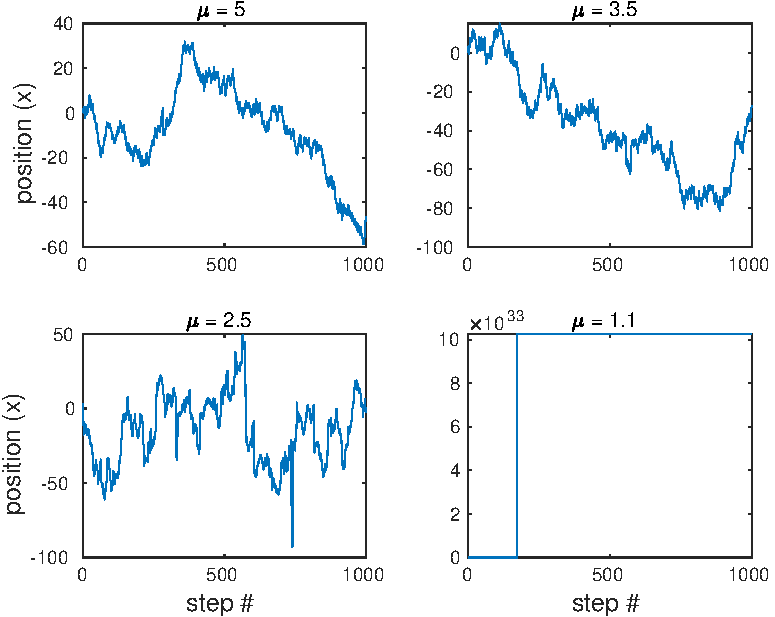
\includegraphics[width=0.8\textwidth]{RandomWalk-PowerLaw}
		\caption[Comparison of different choices of parameter for a random walk with power-law distributed steps]{A realisation of a random walk with power-law step-length distribution, simulated over $1000$ time steps for $x_{\min}=1$ and four different choices of parameter $\mu$. The top-left ($\mu=5$) and top-right ($\mu=3.5$) plots correspond to Brownian motion in the scaling-limit, and the bottom-left ($\mu=2.5$) and bottom-right ($\mu=1.1$) are L\'{e}vy flights.}
		\label{fig:RandomWalk-PowerLaw}
	\end{figure}

\end{subsection}


\end{section}
\FloatBarrier